\documentclass[11pt,a4paper, twocolumn,
swedish, english %% Make sure to put the main language last!
]{article}
\pdfoutput=1

%% Andréas's custom package 
%% (Will work for most purposes, but is mainly focused on physics.)
\usepackage{custom_as}

%% Figures can now be put in a folder: 
\graphicspath{ {figures/} %{some_folder_name/}
}

%% If you want to change the margins for just the captions
\usepackage[margin = 10pt]{caption}

%% To add todo-notes in the pdf
\usepackage[%disable  %%this will hide all notes
]{todonotes} 

%% Change the margin in the documents
\usepackage[
            top    = 2.5cm,              %% top margin
            bottom = 2.5cm,              %% bottom margin
             left   = 1.2cm, right  = 1.2cm %% left and right margins
]{geometry}


%% If you want to change the formatting of the section headers
%\renewcommand{\thesection}{...}

\newcommand{\rr}{\mathrm{r}}

%%%%%%%%%%%%%%%%%%%%%%%%%%%%%%%%%%%%%%%%%%%%%%%%%%%%%%%%%%%%%%%%%%%%%%
\begin{document}%% v v v v v v v v v v v v v v v v v v v v v v v v v v
%%%%%%%%%%%%%%%%%%%%%%%%%%%%%%%%%%%%%%%%%%%%%%%%%%%%%%%%%%%%%%%%%%%%%%


%%%%%%%%%%%%%%%%%%%% vvv Internal title page vvv %%%%%%%%%%%%%%%%%%%%%
\title{SALSA project report}
\author{Andréas Sundström}
\date{2017-11-29}


\twocolumn[
\begin{@twocolumnfalse}
\maketitle
\begin{abstract}
\noindent
Observations, in the Galactic longitude range of $l=20^\circ$ to
$l=210^\circ$, made with the SALSA 2.3\,m radio telescopes at Onsala
Space Observatory of atomic hydrogen (HI) have been used to determine
a rotation curve of the Milky Way and a mapping of the HI cloud
positions. The rotation curve was determined under the assumptions
that all orbits are circular, and that there is always one cloud with
its orbit tangential to the line of sight. Next the mapping of HI
clouds was med under the further assumption that all orbital
velocities are the same at 220\,km/s. The Earth's orbit around the sun
have not been taken into account in any of the calculations or
measurements. 
\end{abstract}
\end{@twocolumnfalse}
]


%%%%%%%%%%%%%%%%%%%% ^^^ Internal title page ^^^ %%%%%%%%%%%%%%%%%%%%%
%% If you want a list of all todos
%\todolist

\section{Introduction}
The interstellar medium (ISM) contains clouds, among others, atomic
hydrogen HI, which trough quantum mechanical hyperfine structure
electronic transitions emits electromagnetic radiation with a
frequency of about 1420\,MHz corresponding to a wavelength of
21\,cm. This frequency then gets Doppler shifted depending on the
relative radial velocity between us and the cloud. Therefore by
observing the frequency spectrum of the incoming radiation in the
21\,cm band, it is possible to determine the presence and relative
radial velocity of clouds in the line of sight.
Once a rotation curve has been established, it can be used to
determine the positions of these clouds.

In this report we use the SALSA 2.3\,m radio telescopes a Onsala Space
Observatory to scan a portion of the Galaxy, that is visible from Onsala,
in the 21\,cm band to find HI clouds. The Doppler shift is then used
to calculate the radial velocity of these clouds, as seen from
Earth. This is then used to determine the rotation curve and the
positions of the observed clouds.

\subsection{Galactic coordinates and measurements}
The Galactic longitude, $l$, of an object is the angle, as seen from
us, in the plane of the Galactic disc between the Galactic center (GC)
and the object in question. The Galactic latitude is measured as the
angle above the Galactic plane. 

\begin{figure}\centering
\resizebox{0.5\linewidth}{!}{
\input{figures/geom.pdf_t}}
\caption{The geometry of an HI measurement, as seen in the plane of
  the Galaxy. If there is a cloud on Galactic longitude $l$ on a circular
  orbit the observed radial velocity is $V_\rr=V\cos\alpha-V_0\sin l$. }
\label{fig:geom}
\end{figure}

Given the geometry of \figref{fig:geom}, the law of sines gives the
relation
\begin{equation}\label{eq:sine-law}
\frac{\sin l}{R_0}=\frac{\sin\beta}{R}
\end{equation}
Assuming circular orbits further gives $\beta=\alpha-\pi/2$.
This together with \eqref{eq:sine-law} means that observed radial
velocity has to be
\begin{equation}\label{eq:Vr}
V_\rr=V\cos\alpha-V_0\sin l
=\sin(l)\qty[\tfrac{R}{R_0}V-V_0].
\end{equation}
This is one equation with two unknowns\footnote{We already know 
  $R_0=\unit[8.5]{kpc}$ and $V_0=\unit[220]{km/s}$ from the SALSA
  Project documentation, to be found at
  \url{https://vale.oso.chalmers.se/salsa/support}.}.
To solve this we (highly dubiously) assume that the clouds we observe
having the highest radial velocity, $V_\rr$, are on a trajectory
tangent to our line of sight ($\alpha=0$). The justification for this
that in each direction looking into the Galaxy, we tend to observe two
or three clouds and therefor it is possible that one of those clods
have $\alpha=0$. If $\alpha=0$ then \eqref{eq:sine-law} yields
$R_0/R=\sin(l)$, or in other words
\begin{equation}\label{eq:Vrmax}
V=V_{\rr,\max}+V_0\sin l.
\end{equation}
We can now determine both $V$ and $R$ together, which makes it
possible to find  the rotation curve.

This is however only possible for when looking in towards the center
of the Galaxy, $0<l<\pi/2$ (or $3\pi/2<l<2\pi$), otherwise the
assumption of trajectories tangential to the line of sight can not be
fulfilled. For $\pi/2<l<3\pi/2$, which also implies $R>R_0$, we cannot
observe the orbital velocity. Instead we just have to blindly hope
that the observed rotation curve extrapolates nicely to $R>R_0$.



\subsubsection{Position determination and ambiguity}
Assuming that we managed to get a rotation curve $V(R)$, and that it
can be extrapolated to all $R$, the position of the observed cloud can
be determined by first inverting \eqref{eq:Vr} to get $R$. Once we
have $R$, we need $d$ to fully determine the position of the HI
cloud.

By the law of cosines, we have
\begin{equation}
R^2=R_0^2+d^2-2R_0d\cos l,
\end{equation}
which inverts to
\begin{equation}\label{eq:d}
d=R_0\cos l \pm\sqrt{R^2-R_0^2\sin^2l}.
\end{equation}
For $R>R_0$ it is clear that one of the above solution must be
negative, hence the cloud position is uniquely determined.
If, on the other hand, $R<R_0$ (which implies that $0<l<\pi/2$ or
$3\pi/2<l<2\pi$) there might be two positive solutions, which means
that $d$ could be ambiguous. This happens when 
\begin{equation}
R_0\cos l>\sqrt{R^2-R_0^2\sin^2l}.
\end{equation}
Since the premise was that $0<l<\pi/2$ or $3\pi/2<l<2\pi$ we have
$\cos l>0$, hence we have ambiguity when
$R_0^2\cos^2l>R^2-R_0^2\sin^2l$ which is equivalent to
\begin{equation}
R_0^2>R^2.
\end{equation}
This is always true with the initial assumption $R<R_0$. Hence the
position is \emph{ambiguous} for all $R<R_0$ and \emph{unique} for all
$R>R_0$. This type of ambiguity is illustrated in \figref{fig:geom} by
the position marked by the dotted line.

\section{Method}
The SALSA 2.3\,m radio telescopes at Onsala Space Observatory were
used to observe the frequency spectrum at around 21\,cm for a range of
different Galactic longitudes. In The control software of these
telescopes have the feature to track on Galactic coordinates. Each
observation was med with an integration time of 50\,s. Then the Matlab
class provided on the SALSA web page\footnotemark{} was used to further
analyze the frequency spectrum by subtracting a background level and
then fitting Gaussian curves to the remaining peaks. The curve fitting
was mostly done via the automatic function provided in the class,
however all fits were manually reviewed and those who were obviously
wrong were corrected through manual fitting.
\footnotetext{\url{https://vale.oso.chalmers.se/salsa/software}}

The rotation curve was found (\figref{fig:rot}) using
\eqref{eq:Vrmax}. It was then used to make the assumption that all 
orbital velocities are constant $V=V_0=\unit[220]{km/s}$. This was
then used to find 
\begin{equation}\label{eq:R}
R=\frac{R_0V_0\sin l}{V_0\sin l -V_\rr}, 
\end{equation}
which could then be used in \eqref{eq:d} to determine the position of
the cloud. All clouds were assumed to be at the $+$ solution of
\eqref{eq:d}, since that is the only physical solution when
$R>R_0$. For $R<R_0$ the clouds were marked out as ambiguous, and could
be at the $-$ solution instead.

For the Galactic longitude of $l=50^\circ$, we were able to resolve
the ambiguity problem for one cloud by observing how the peaks were
affected when observing at Galactic latitudes of $b=0^\circ, 5^\circ$
and $10^\circ$. 

\section{Results and Discussion}
\begin{figure}\centering
\includegraphics[width=1\linewidth]{rotation_curve.eps}
\caption{Velocity curve for HI clouds in the Milky Way, as observed
  between $20^\circ{-}85^\circ$ Galactic longitude with $5^\circ$
  increments. These velocities are calculated using the circular orbit
  assumption, as well as assuming that the cloud with the highest
  radial velocity is moving tangent to the line of sight.}
\label{fig:rot}
\end{figure}

\begin{figure}\centering
\includegraphics[width=1\linewidth]{gas_clouds.eps}
\caption{Positions of atomic hydrogen (HI) clouds in the Milky Way,
  spanning from Galactic longitude $l=20^\circ$ to $l=210^\circ$. The
  $X$ and $Y$ axes are set with the origin at the Galactic center; and
  the dotted lines represent distances between 4\,kpc and 20\,kpc, in
  2\,kpc steps, from the Galactic center. Some type of Galactic arm
  structures can be discerned. The positions are calculated using the
  assumptions that all clouds have circular orbits and that their
  orbital velocities are $V_0=\unit[220]{km/s}$. For the clouds with
  an orbital radius of $R<R_0=\unit[8.5]{kpc}$ (marked with red
  crosses) there are two possible solutions to their position. This
  ambiguity problem have been resolved for one cloud on $l=50^\circ$ 
  (red ring, correct position filled in). }
\label{fig:clouds}
\end{figure}

\begin{figure}\centering
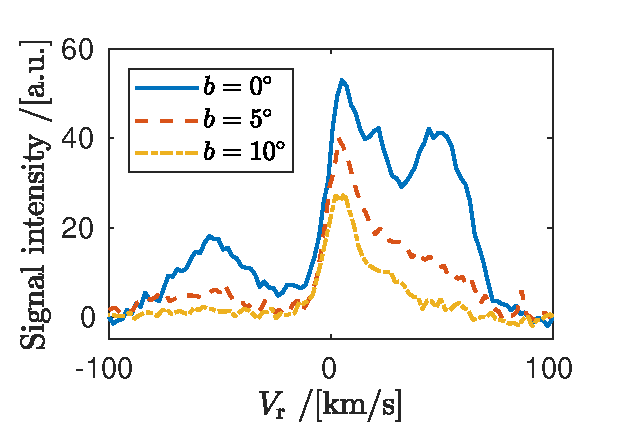
\includegraphics[width=1\linewidth]{ambiguity.eps}
\caption{Velocity spectra, calculated from Doppler shift, to resolve
  the ambiguity problem for $l=50^\circ$. By observing that that the
  peak near $V=0$ remains for different Galactic latitudes, $b$, we
  can conclude that this gas cloud has to be much closer to us than
  the two others which can be seen at $b=0^\circ$. }
\label{fig:ambiguity}
\end{figure}

The rotation curve found in this observation is shown in
\figref{fig:rot}. As we can see the orbital velocities, $V$, seems to
maybe tend towards a roughly constant value of
$V=V_0=\unit[220]{km/s}$, which is the assumption made to create the
map of the gas clouds in \figref{fig:clouds}. We do however also see
that this  assumption fails for $R<\unit[5]{kpc}$, which means that
the positions of those clouds in \figref{fig:clouds} should be
considered as highly uncertain.

As shown before, all positions with $R<R_0=\unit[8.5]{kpc}$ are
ambiguous and therefore marked out with red crosses in
\figref{fig:clouds}. They should therefore not be considered as actual
positions of the clouds. In the case of $l=50^\circ$, we measured not
only in the Galactic plane, but also $5^\circ$ and $10^\circ$ above the
Galactic plane to see whether or not a cloud was very near us, and in
that way try to resolve the ambiguity problem. The results of these
measurements are shown in \figref{fig:ambiguity}. As can be seen there,
the peak near $V_\rr=\unit[0]{km/s}$ is least affected by the higher
Galactic latitudes, indicating that the could corresponding to that
peaks is quite close to us. Using the observed $V_\rr$, we could
determine that the orbital radius of this cloud is
$R=\unit[8]{kpc}$. By studying the clouds on the $l=50^\circ$ line of
sight, dashed line in \figref{fig:clouds}, we can conclude that there
are two positions at $l=50^\circ$ and $R=\unit[8]{kpc}$ and they are
quite far apart. The last observation makes it clear that the cloud
has to be on the closer position, marked with a filled in red circle.


\subsection{Uncertainties}
\textsl{In the words of Monty Python:} \textit{When you assume, you
  make an ass out of u and me.}

As mentioned before we assumed that, when we are observing in
$0<l<\pi/2$, we always see a cloud on a path tangential to its
orbit. This was done to be able to draw up the rotation curve in
\figref{fig:rot}. Note that only clouds with $Y>0$ can satisfy our
assumption. 
This was purely based on the hope that there would
be enough clouds in the region of interest that the probability of
seeing one straight down its trajectory would be very likely.
However as we can see in \figref{fig:clouds}, there are not that many
clouds in that region; as they are marked out now almost none of them
satisfy our assumption, but their positions are ambiguous which means
that some of the clouds have to be on the closer possible position
which would put them on $Y>0$ -- i.e. it's at least not impossible to
fulfill the assumption. Still however, this assumption needs more
backing up than is presented in this report. 

The next assumption was that all clouds have orbitals velocities of
$V=V_0=\unit[220]{km/s}$. The assumption is based on the observed
rotation curve in \figref{fig:rot}. We can see that this seems to be
roughly true for the data points between $R=\unit[6]{kpc}$ and
$R=\unit[8.5]{kpc}$. It is however expected that the orbital velocity
should drop as $R$ gets small, as there will be less mass inside
$R$. This dose however mean that the orbital radii of the clouds found
to be at $R<\unit[5]{kpc}$, using \eqref{eq:R}, are wrong, but as
their positions are ambiguous any way that is not a very big
problem. The more pressing problem here is the fact that the data,
which from the very beginning is questionable (see the previous
paragraph) from the small interval of $R=\unit[6]{kpc}$ to
$R=\unit[8.5]{kpc}$ is extrapolated to as far out as
$R=\unit[19]{kpc}$.

Another source of uncertainty is the orbital velocity of the Earth
around the Sun, which is about $\unit[30]{km/s}$ or almost 14\,\% of
$V_0$ -- i.e. \emph{not} negligible. This is a large source of error
since it has not been taken into account in any of the above
calculations. This not only affects the results from \eqref{eq:Vrmax}
and \eqref{eq:R}, which is the mathematical bedrock of this report,
but also how their form. Since velocity is a vector, and our total
velocity relative to the Galactic center is the vector sum of the
Earth's orbital velocity around the Sun and the Sun's orbital velocity
around the Galactic center, the starting assumption \eqref{eq:Vr} is
invalid and has to be changed, which in turn changes the form of all
the following equations.



\section{Conclusions}
In conclusion the SALSA 2.3\,m radio telescope at Onsala Space
Observatory have been used to observe atomic hydrogen, HI, in a range
of Galactic longitudes from $l=20^\circ$ to $l=210^\circ$. These
observations have been used to determine a rotation curve of the Milky 
Way, under the assumptions that their orbits are circular and that
their orbital velocities are parallel to the line of sight. Clouds at
(assumed) orbital radii between 6\,kpc and 8.5\,kpc are seen to have
almost constant orbital velocities of around 220\,km/s.

Assuming that all of the clouds in the Galaxy also have the same
orbital velocity was then used to map out the positions of all
observed clouds. Clouds closer to the Galactic center than us have
ambiguous positions, but for one cloud on $l=50^\circ$ this ambiguity
was resolved by studying how the signal changed when observing out
from the Galactic disc.

There were several assumptions made to arrive at the results presented
in this report. Some of which are more severe than others. The overall
the level of uncertainty, due to the ingoing assumptions, is highly
unsatisfactory in all the results presented. This can not be mended
with better equipment. 










%%%%%%%%%%%%%%%%%%%%%%%%%% The bibliography %%%%%%%%%%%%%%%%%%%%%%%%%%
%\newpage
%% This bibliography uses BibTeX
%\bibliographystyle{ieeetr}
%\bibliography{references}%requires a file named 'references.bib'
%% Citations are as usual: \cite{example_article}

%%%%%%%%%%%%%%%%%%%%%%%%%%%%% Appendices %%%%%%%%%%%%%%%%%%%%%%%%%%%%%

%%%%%%%%%%%%%%%%%%%%%%%%%%%%%%%%%%%%%%%%%%%%%%%%%%%%%%%%%%%%%%%%%%%%%%
\end{document}%% ^ ^ ^ ^ ^ ^ ^ ^ ^ ^ ^ ^ ^ ^ ^ ^ ^ ^ ^ ^ ^ ^ ^ ^ ^ ^ ^
%%%%%%%%%%%%%%%%%%%%%%%%%%%%%%%%%%%%%%%%%%%%%%%%%%%%%%%%%%%%%%%%%%%%%%


%%% Local Variables:
%%% mode: latex
%%% TeX-master: t
%%% End:

%  LocalWords:  hyperfine Onsala kpc
